\documentclass[11pt]{article}
\usepackage[utf8]{inputenc}
\usepackage[T1]{fontenc}
\usepackage[spanish,es-tabla,es-noshorthands]{babel}
\usepackage{graphicx} % Required for inserting images
\usepackage[margin=2cm]{geometry}
\usepackage{booktabs}
\usepackage{float}
\usepackage{caption}
\usepackage{subcaption}
\usepackage{xcolor}
\usepackage{listings}
\usepackage{hyperref}

\graphicspath{{figs/}}
\captionsetup{font=small,skip=4pt}
\setlength{\textfloatsep}{8pt}
\setlength{\intextsep}{8pt}
\usepackage{titling}
\setlength{\droptitle}{-2cm}

\lstset{
  language=Python,
  basicstyle=\ttfamily\small,
  keywordstyle=\color{blue!70!black}\bfseries,
  commentstyle=\color{green!45!black}\itshape,
  stringstyle=\color{red!60!black},
  frame=single,
  breaklines=true,
  showstringspaces=false,
  columns=fullflexible,
  literate={á}{{\'a}}1 {é}{{\'e}}1 {í}{{\'i}}1 {ó}{{\'o}}1 {ú}{{\'u}}1 {ñ}{{\~n}}1
}

\title{Mini3E2 Informe\\[0.3em]\large Miniproyecto 3: Clasificación de animales, Entrega 2}
\author{Daniela Solarte}
\date{Octubre 2026}

\begin{document}

\maketitle

\section{Introducción}

En esta entrega se implementaron los dos primeros descriptores del Miniproyecto 3, uno de color y otro de textura, y se usaron con un clasificador de K vecinos más cercanos (K-NN) para distinguir las cinco especies asignadas al grupo 19: \emph{Castor canadensis}, \emph{Didelphis virginiana}, \emph{Procyon lotor}, \emph{Sciurus niger} y \emph{Urocyon cinereoargenteus}. Se reutilizaron las funciones de la Entrega 1 (\texttt{get\_data} y \texttt{processing}), con rutas relativas a la carpeta \texttt{dataset}. Todas las celdas se ejecutaron sin errores y se superaron todas las pruebas (\texttt{assert}) del enunciado.

\section{Descriptores de color}

La función \texttt{color\_hist} calcula dos tipos de histograma sobre una imagen de tres canales:

\begin{itemize}
  \item \textbf{Concatenado:} un histograma de \texttt{bins} intervalos por canal con \texttt{np.histogram}; los tres se unen en un vector de $3\cdot\texttt{bins}$ posiciones.
  \item \textbf{Conjunto:} un histograma tridimensional con \texttt{np.histogramdd} que cuenta cada combinación de los tres canales; se aplana a un vector de $\texttt{bins}^3$ posiciones.
\end{itemize}

En ambos casos el vector se divide por su suma para que quede normalizado. Siguiendo el tutorial de la semana 11, el rango de los intervalos va del mínimo al máximo de cada canal de la imagen; con esta implementación se obtienen las desviaciones estándar que esperan las pruebas (0,024 para el concatenado y 0,0063 para el conjunto). En la Figura~\ref{fig:hist} se observa que el histograma conjunto es muy disperso: de sus 1000 posiciones, solo unas pocas son distintas de cero.

\begin{figure}[H]
\centering
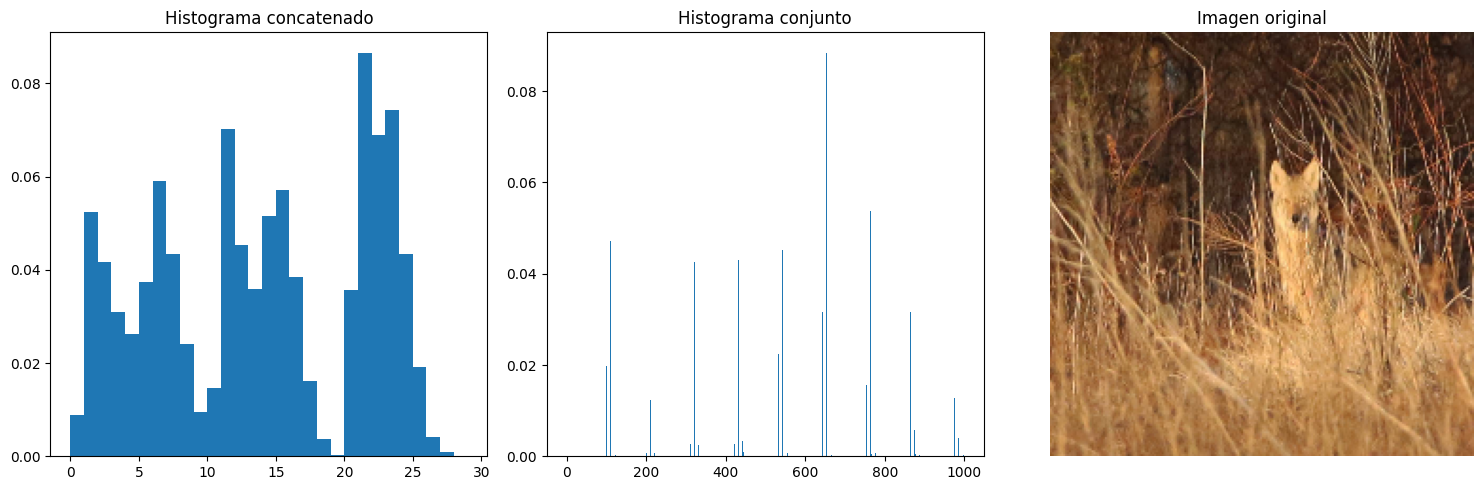
\includegraphics[width=0.85\textwidth]{hist_color.png}
\caption{Histograma concatenado (30 posiciones) y conjunto (1000 posiciones) con 10 bins por canal, para la imagen de prueba de \emph{Canis latrans} en RGB a $224\times224$.}
\label{fig:hist}
\end{figure}

Se calcularon ambos histogramas para las 5163 imágenes de entrenamiento y las 1723 de validación, a $224\times224$, en HSV y con 10 bins por canal. Con cada descriptor se entrenó un \texttt{KNeighborsClassifier} con $k=5$, y se evaluó con \texttt{precision\_recall\_fscore\_support} y promedio \texttt{macro}, que da el mismo peso a cada especie pese al desbalance entre clases (Tabla~\ref{tab:color}).

\begin{table}[H]
\centering
\caption{Métricas promedio (macro) en validación con descriptores de color (HSV, 10 bins, $k=5$).}
\label{tab:color}
\begin{tabular}{lccc}
\toprule
Descriptor & Precisión & Cobertura & F1 \\
\midrule
Histograma concatenado & 0,373 & 0,358 & \textbf{0,351} \\
Histograma conjunto    & 0,356 & 0,344 & 0,336 \\
\bottomrule
\end{tabular}
\end{table}

Ambos modelos superan el umbral de 0,28 del enunciado y el azar para cinco clases (cerca de 0,20), pero quedan lejos de una buena clasificación. El concatenado es ligeramente mejor, posiblemente por la dispersión del conjunto: con 1000 posiciones casi vacías, dos imágenes de colores parecidos pueden caer en celdas distintas y quedar lejos en la distancia euclidiana de K-NN. Además, las cinco especies tienen pelajes cafés o grises parecidos y el fondo ocupa la mayor parte de la imagen. Por último, como el rango de los bins depende de cada imagen, un mismo bin no representa exactamente el mismo color en todas, lo que también puede reducir el desempeño.

\section{Descriptores de textura}

\subsection{Banco de filtros y diccionario de textones}

El banco de filtros se cargó con \texttt{loadmat} y contiene 18 filtros de $49\times49$. La función \texttt{filter\_map} convierte la imagen a escala de grises si tiene tres canales, aplica cada filtro con \texttt{correlate2d} en modo \texttt{"same"} y apila las 18 respuestas como canales de una sola imagen. Cada filtro resalta estructuras con su misma orientación; por ejemplo, el filtro 10, diagonal, responde con fuerza a los tallos de pasto inclinados (Figura~\ref{fig:filtros}a).

Para construir el diccionario se tomaron 25 imágenes de entrenamiento (5 por clase, elegidas al azar con la semilla 19) a $256\times256$ en escala de grises. La función \texttt{pixel\_dataset} convierte cada píxel en un vector de 18 respuestas, lo que da $256\cdot256\cdot25 = 1\,638\,400$ píxeles. Con ellos se entrenó un \texttt{KMeans} con $K=25$ textones. La función \texttt{texture\_map} predice el textón de todos los píxeles de una imagen al mismo tiempo y reconstruye un mapa de $256\times256$ (Figura~\ref{fig:filtros}b), y \texttt{texture\_histogram} cuenta la frecuencia de cada textón en un histograma normalizado de 25 bins. En el mapa aparece un marco en los bordes porque \texttt{correlate2d} rellena con ceros fuera de la imagen, lo que altera la respuesta de los filtros en una franja de unos 24 píxeles.

\begin{figure}[H]
\centering
\begin{subfigure}[b]{0.46\textwidth}
  \centering
  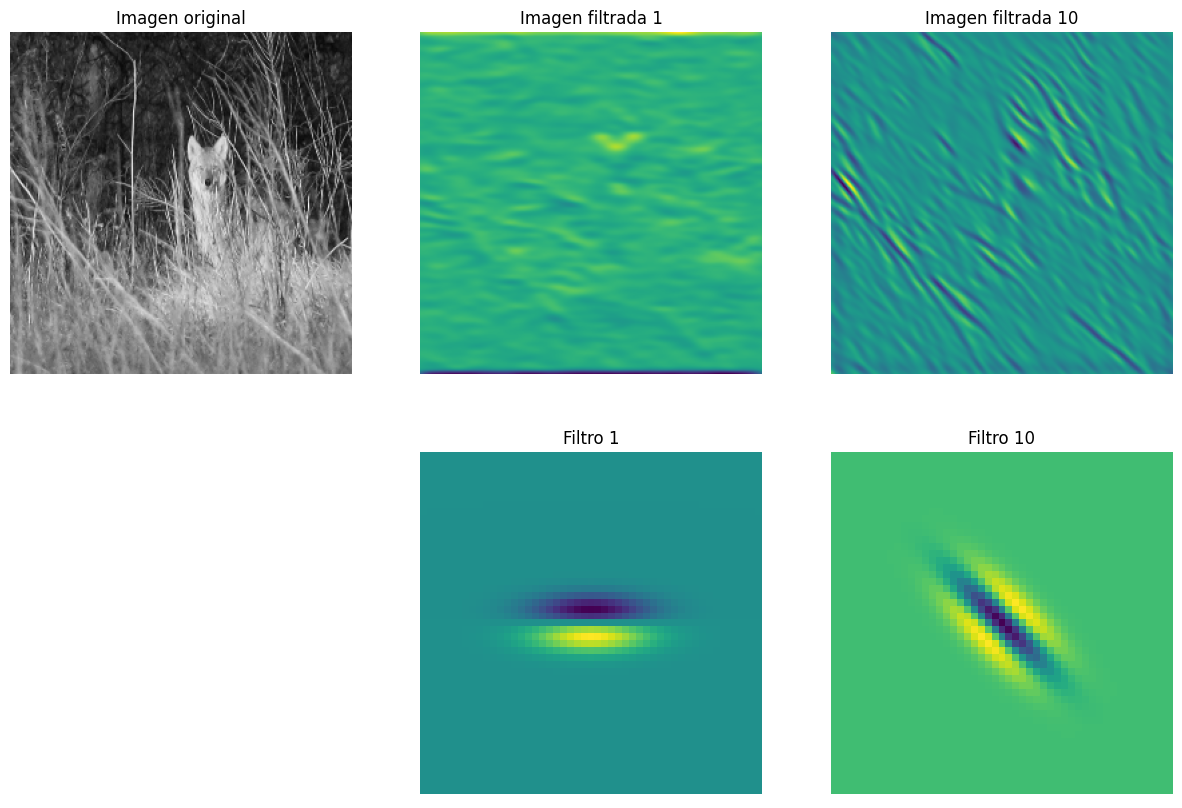
\includegraphics[width=\textwidth]{filtros.png}
  \caption{Imagen en gris, respuestas a los filtros 1 y 10 (arriba) y los filtros (abajo).}
\end{subfigure}
\hfill
\begin{subfigure}[b]{0.5\textwidth}
  \centering
  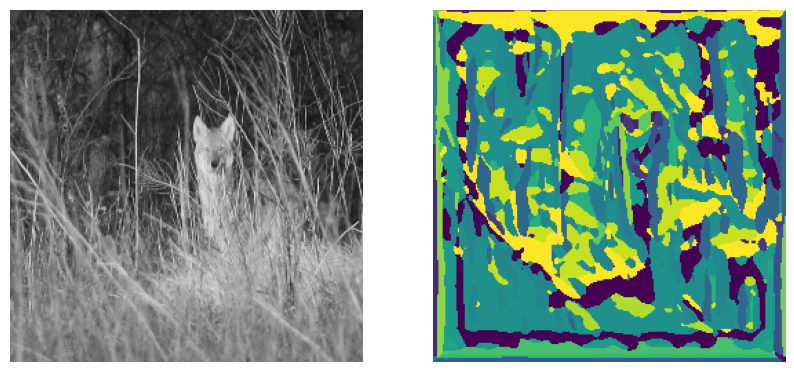
\includegraphics[width=\textwidth]{textones.png}
  \caption{Imagen de prueba y su mapa de 25 textones.}
\end{subfigure}
\caption{Banco de filtros y mapa de textones para la imagen de prueba de \emph{Canis latrans} ($256\times256$).}
\label{fig:filtros}
\end{figure}

\subsection{Clasificación}

Se extrajo el histograma de textones de 150 imágenes de entrenamiento (30 por clase) y de 50 de validación (10 por clase), y los descriptores se guardaron con \texttt{pickle}. Con ellos se entrenó un K-NN con $k=5$. La Tabla~\ref{tab:textura} presenta las métricas por clase y la Figura~\ref{fig:textura} la matriz de confusión.

\begin{figure}[H]
\centering
\begin{minipage}[c]{0.55\textwidth}
\centering
\captionof{table}{Métricas en validación con textura (25 textones, $k=5$, 10 imágenes por clase).}
\label{tab:textura}
\small
\begin{tabular}{lccc}
\toprule
Clase & Precisión & Cobertura & F1 \\
\midrule
\emph{C. canadensis}        & 0,250 & 0,500 & 0,333 \\
\emph{D. virginiana}        & 0,200 & 0,100 & 0,133 \\
\emph{P. lotor}             & 0,250 & 0,200 & 0,222 \\
\emph{S. niger}             & 0,400 & 0,400 & 0,400 \\
\emph{U. cinereoargenteus}  & 0,286 & 0,200 & 0,235 \\
\midrule
\textbf{Promedio (macro)}   & \textbf{0,277} & \textbf{0,280} & \textbf{0,265} \\
\bottomrule
\end{tabular}
\end{minipage}
\hfill
\begin{minipage}[c]{0.42\textwidth}
\centering
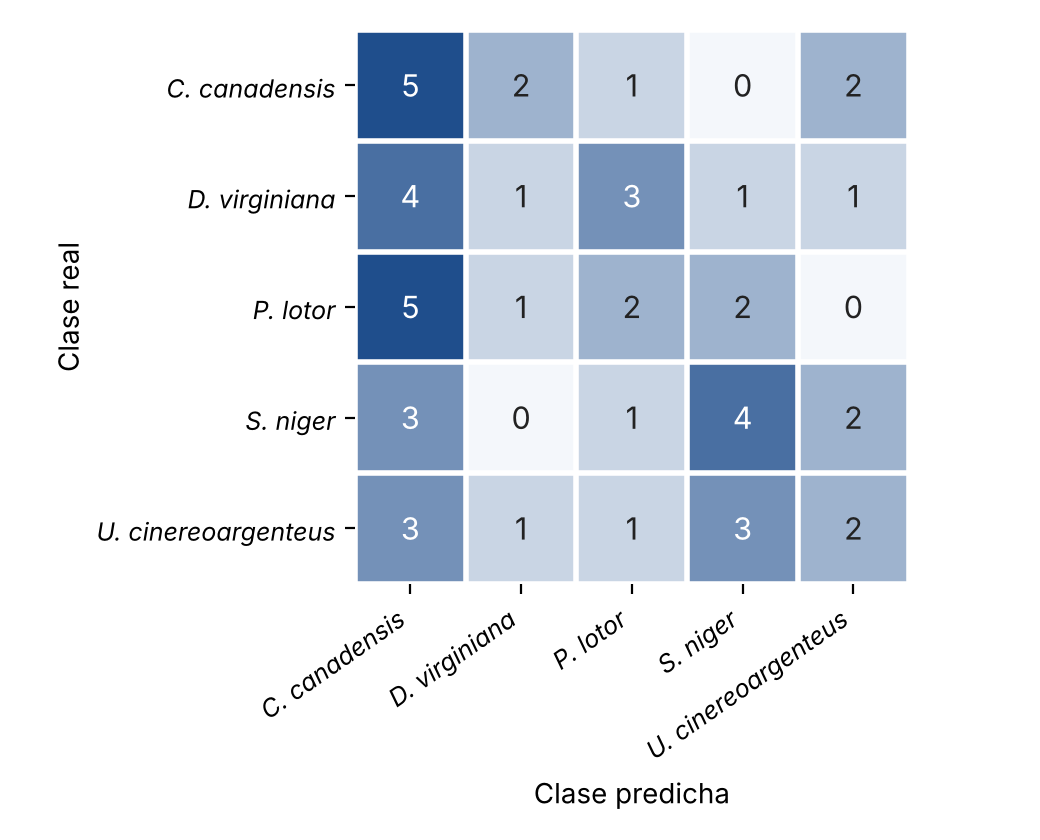
\includegraphics[width=\textwidth]{confusion_textura.png}
\captionof{figure}{Matriz de confusión del descriptor de textura en validación (50 imágenes).}
\label{fig:textura}
\end{minipage}
\end{figure}

El F1 promedio de 0,265 supera el umbral de 0,16 del enunciado. \emph{Sciurus niger} es la clase mejor reconocida. \emph{Didelphis virginiana} es la peor: solo una de sus diez imágenes se clasificó bien y cuatro se confundieron con \emph{Castor canadensis}. La matriz de confusión muestra que el modelo asigna esa clase a 20 de las 50 imágenes, lo que explica por qué su cobertura es alta (0,50) y su precisión baja (0,25). Como hay solo diez imágenes de validación por clase, cada acierto o error cambia la cobertura en 0,10, así que estas métricas por clase son muy variables.

\section{Comparación y costo computacional}

Con el color se obtuvo un F1 mayor (0,351) que con la textura (0,265), pero la comparación no es directa: el modelo de color se entrenó con 5163 imágenes y se evaluó con 1723, mientras que el de textura usó 150 y 50. La diferencia también refleja el costo de cada descriptor. Calcular los histogramas de color de las 6886 imágenes tomó unos 5 minutos. En cambio, con \texttt{correlate2d} y filtros de $49\times49$, la colección de píxeles de las 25 imágenes tardó unos 17 minutos y los descriptores de las 200 imágenes de clasificación, cerca de 55 minutos. Este costo justifica la versión de \texttt{filter\_map} con \texttt{torch} del final del notebook.

\section{Conclusiones}

\begin{itemize}
  \item Se implementaron los histogramas de color concatenado y conjunto, el banco de filtros, el diccionario de textones con KMeans y el histograma de textones, y se superaron todas las pruebas del notebook.
  \item Con K-NN, el histograma de color concatenado en HSV obtuvo el mejor F1 (0,351), seguido del conjunto (0,336). Ambos superan el azar, pero el color por sí solo no basta, porque las especies y los fondos comparten tonos similares.
  \item El descriptor de textura alcanzó un F1 de 0,265 con solo 150 imágenes de entrenamiento y tiende a predecir \emph{Castor canadensis} en exceso.
  \item El descriptor de textura es mucho más costoso de calcular. Para las siguientes entregas conviene usar la versión con \texttt{torch}, entrenar con más imágenes y probar la combinación de color y textura.
\end{itemize}

\begin{flushright}
\small Realizado en \LaTeX
\end{flushright}

\end{document}
